\newpage
\section{Noise, General Measurement, and Qubit Decoherence}

\subsection{Classes of Errors in a Circuit Model}
\begin{enumerate}\small
    \item State preparation. Need to couple qubits to other items (cavities, controls, measurement devices) and apply complex protocols to ensure a fast reset. 
    \item Gate imperfection. Imprecise amplitude, phase, or duration of microwave pulses, and qubit frequency fluctuations. 
    \item Measurement errors. Limited integration time, measurement induced decoherence, and amplifier and detector noise. 
    \item Qubit decoherence. Environment induced relaxation, heating, and dephasing, as well as crosstalk, unwanted interaction between the qubits.
\end{enumerate}

\subsection{Insights from Classical Noise}
We can model the single-stage process by a probability $p$ for the bit to flip, and a probability $1-p$ for the bit to remain the same. 

\begin{figure}[!htb]
    \centering
    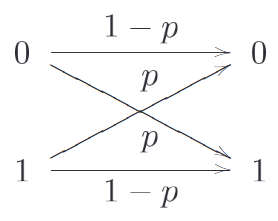
\includegraphics[width=0.2\textwidth]{QI11/single-stage process}
    \caption{single-stage process}
\end{figure}

Therefore, a classical state is described by a vector of probabilities. We only need to know the evolution matrix (or matrix of transition probabilities), which states that
\begin{align*}
    p(Y=y)=\sum_x p(Y=y|X=x)p(X=x)
\end{align*}
The previous example can be expressed in a matrix form as
\begin{align*}
    \begin{bmatrix}
        p(Y=0)\\p(Y=1)
    \end{bmatrix}=\begin{pmatrix}
        1-p & p \\ p & 1-p
    \end{pmatrix}\begin{bmatrix}
        p(X=0)\\p(X=1)
    \end{bmatrix}
\end{align*}
or, in a short notation
\begin{align*}
    \vec{p}_Y=E\vec{p}_X\equiv\mathcal{E}(\vec{p}_X)
\end{align*}
The evolution matrix E requires
\begin{enumerate}\small
    \item all the entries of E must be non-negative; the positivity condition resulting in positive probabilities only,
    \item all the columns of E must sum to one; the completeness condition resulting in conserved total probability.    
\end{enumerate}

To model these effects, we use the density matrix language to describe probabilistic quantum states and study their evolution in the presence of an environment.

\subsection{Quantum Operation Formalism}
\subsubsection{Density Matrices and Quantum Operations}
Quantum systems are inherently probabilistic. Measurements or random perturbations lead to probabilistic outcomes, which are described in terms of density matrices. 

For example, to prepare a quantum state $\ket{\psi}$, a noisy quantum system likely produces a random distribution of quantum states, i.e., $\ket{\psi_i}$ with probability $p_i$ , due to imprecise controls or environmental noise. We use the density matrix
\begin{align*}
    \rho=\sum_i p_i \ket{\psi_i}\bra{\psi_i}
\end{align*}
to describe the mixed state, as oppose to $p_0=\ket{\psi}\bra{\psi}$. 

The quantum operation formalism is a general tool for describing the evolution of quantum systems. Similar to how classical states evolves, quantum states transform as
\begin{align*}
    \rho'=\mathcal{E}(\rho)
\end{align*}
The map $\mathcal{E}$ in this equation is a \textbf{quantum operation}.

The dynamics of a closed quantum system are described by a unitary transform. An unitary evolution is a quantum operation:
\begin{align*}
    \mathcal{E}(\rho)=U\rho U^\dagger
\end{align*}
which results from $\ket{\psi_i'}=U\ket{\psi_i}$. 

On the other hand, measurement is also a quantum operation. However, the process of measurement is irreversible and probabilistic. 

For the computational basis (projective) measurement, we take $M_1 = \ket{0}\bra{0}$ and $M_2 = \ket{1}\bra{1}$. If the initial state is $\ket{\psi_i}$, we obtain the outcome m with probability
\begin{align*}
    p_i^m=|\braket{m|\psi_i}|^2=|M_m\ket{\psi_i}|^2=\braket{\psi_i|M_m^\dagger M_m|\psi_i}
\end{align*}
and the state after the measurement is
\begin{align*}
    \ket{\psi_i^m}=\frac{M_m\ket{\psi_i}}{|M_m\ket{\psi_i}|}=\frac{M_m\ket{\psi_i}}{\sqrt{\braket{\psi_i|M_m^\dagger M_m|\psi_i}}}
\end{align*}
The total probability of obtaining $m$ is
\begin{align*}
    \rho_m&=\sum_i p_i p_i^m=\sum_i p_i \braket{\psi_i|M_m^\dagger M_m|\psi_i}\\
    &=\sum_i p_i \mathrm{Tr}(M_m^\dagger M_m \ket{\psi_i}\bra{\psi_i})\\
    &=\mathrm{Tr}(M_m^\dagger M_m \rho)=\mathrm{Tr}(M_m\rho M_m^\dagger)
\end{align*}
Similarly, the density matrix of the resulting state is
\begin{align*}
    \rho'\equiv\mathcal{E}(\rho)&=\sum_i p_i\left[ \sum_m p_i^m \ket{\psi_i^m}\bra{\psi_i^m} \right]\\
    &=\sum_m M_m \rho M_m^\dagger
\end{align*}

So far, we have shown that the quantum operation formalism is a general tool for describing the evolution of quantum systems, including unitary transformations $\mathcal{E}=U\rho U^\dagger$ and measurements $\mathcal{E}(\rho)=M_m \rho M_m^\dagger$. 

We can now develop a general theory of quantum operations, motivated by the physical reality of a system coupled to an environment. 

As one can anticipate from the previous discussions on unitary transformations and measurements, quantum operations can be represented in an elegant \textbf{operator-sum representation}.

\subsubsection{Operator-Sum Representation}
Assume the system $S$ is part of a larger and closed system, which also includes the environment $E$ . For practical interest, we can assume the initial density matrix is separable
\begin{align*}
    \rho=\rho_S(0)\otimes\rho_E(0)
\end{align*}
where $\rho_E(0)\ket{e_0}\bra{e_0}$ is a pure state. Let $\ket{e_k}$ be orthonormal basis for the environmental state space. 

The system and the environment are coupled by a time-independent Hamiltonian $H$, leading to a unitary time evolution of the total system.

We then take a partial trace over the environment, which allows us to obtain the reduced state of the system alone.

\begin{figure}[!htb]
    \centering
    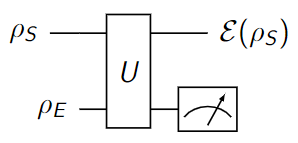
\includegraphics[width=0.36\textwidth]{QI11/a partial trace over the environment}
    \caption{a partial trace over the environment}
\end{figure}

As illustrated in the figure, the partial trace can be represented by a measurement in $\ket{e_k}$ basis of the environment (qubits). However, we do not acquire the outcome $k$ from the measurement.

Put together, with the time evolution operator $U(t)=e^{iHt/\hbar}$, the evolution of the reduced density matrix (which we care) is
\begin{align*}
    \rho_S(t)&=\mathrm{Tr}_E\left\{ U(t)\left[ \rho_S(0)\otimes \ket{e_0}\bra{e_0} \right] U^\dagger (t) \right\}\\
    &=\sum_k \braket{e_k | U(t) | e_0}\rho_S(0)\braket{e_0| U^\dagger(t) |e_k}\\
    &=\sum_k E_k \rho_S(0)E_k^\dagger
\end{align*}
where $E_k=\braket{e_k| U(t) |e_0}$ are known as the \textbf{Kraus operator} acting on the Hilbert space of the system. 

The Kraus operators satisfy the completeness constraint $\displaystyle \sum_k E_k^\dagger E_k=1$, if no information about what occurred in the process is obtained by measurement.

The Kraus operators encode all the available information about the initial state of the environment and about the dynamics of the system-environment coupling. Therefore, the operator-sum representation describes the dynamics of the system without having to explicitly consider properties of the environment.

Consequently, the reduced density matrix of the system satisfies:
\begin{itemize}
    \item $\rho_S(t)$ is Hermitian.
    \item $\rho_S(t)$ has unit trace.
    \item $\rho_S(t)$ is positive.
\end{itemize}
These properties can be compared to the positivity and completeness conditions in the description of classical noise.

In general, the evolution is not unitary, and $\rho_S(t)$ is in a mixed state after partial trace. There is an arrow of time, i.e., $E_k$ are not invertible. 

\subsubsection{General Measurements}
The structure of the operator-sum representation is similar to the quantum operation of projective measurement
\begin{align*}
    \mathcal{E}_m(\rho)=\sum_m M_m \rho M_m^\dagger
\end{align*}
where $P_m\equiv M_m=M_m^\dagger$ is a projector. This allows us to interpret $\{ E_k \}$ as a general measurement of the qubit system, with a projective measurement $I^S \otimes P_k^E$ on the composite system. 

The quantum operation takes the state $\rho_S$ and randomly replaces it by
\begin{align*}
    \rho_k=\frac{E_k\rho E_k^\dagger}{\mathrm{Tr}(E_k\rho E_k^\dagger)}
\end{align*}
with probability $\mathrm{Tr}(E_k\rho E_k^\dagger)$. The result of $\rho_k$ is the direct consequence of the outcome $k$ from the measurement of the environment.

In theoretical study, projective measurements are usually enough because most physical system can only be measured in a very coarse manner.

In qubit readouts, however, we aim for an exquisite level of control over the measurements that can be done. Such a real measurement involves an ancilla system (i.e., an environment); in the qubit-cavity case, it is the cavity.

Therefore, we need to consider, in general, the unitary evolution of the composite quantum system and the measurement of the ancilla system. The index $k$ labels the readout of the ancilla system.


\subsection{Qubit Decoherence}
In general, superconducting qubits are not identical and contains (magnetic) impurities and quasiparticle excitations, hence are subject to various random sources of noise. 

The effects of noise are usually separated into two terms: 
\begin{itemize}\small
    \item Relaxation: transition that change the qubit state.
    \item Dephasing: modulation of transition frequencies which leads to phase randomization.
\end{itemize}

\begin{figure}[!htb]
    \centering
    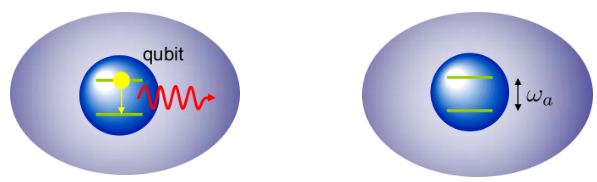
\includegraphics[width=0.42\textwidth]{QI11/The effects of noise}
    \caption{The effects of noise}
\end{figure}

\subsubsection{Amplitude Damping}
The amplitude-damping channel is a schematic model of the decay of an excited state of a qubit due to spontaneous emission of a photon.

We denote the qubit ground state by $\ket{g}$ and the excited state of interest by $\ket{e}$. The ``environment'' is the electromagnetic field, assumed initially to be in its vacuum state $\ket{0}$. After a while, there is a probability p that the excited state has decayed to the ground state and a photon has been emitted, so that the environment has made a transition from the state $\ket{0}$ (``no photon'') to the state $\ket{1}$ (``one photon'').

The unitary evolution $U_{SE}$ of the qubit and environment is
\begin{align*}
    \ket{g}\ket{0}&\rightarrow\ket{g}\ket{0}\\
    \ket{e}\ket{0}&\rightarrow\sqrt{1-p}\ket{e}\ket{0}+\sqrt{p}\ket{g}\ket{1}
\end{align*}
By evaluating the partial trace over the environment, we find the Kraus operators
\begin{align*}
    E_0&=\braket{0|U_{SE}|0}=\begin{pmatrix}
        1 & 0 \\ 0 & \sqrt{1-p}
    \end{pmatrix}\\
    E_1&=\braket{1|U_{SE}|0}=\begin{pmatrix}
        0 & p \\ 0 & 0 
    \end{pmatrix}
\end{align*}
The density matrix evolves as
\begin{align*}
    \rho_S(0)&=\begin{pmatrix}
        \rho_{gg} & \rho_{ge}\\ \rho_{eg} & \rho_{ee}
    \end{pmatrix}\\
    \rho_S(t)&=E_0\rho_S(0)E_0^\dagger+E_1\rho_S(0)E_1^\dagger\\
    &=\begin{pmatrix}
        \rho_{gg} & \sqrt{1-p}\rho_{ge}\\ \sqrt{1-p}\rho_{eg}& (1-p)\rho_{ee}
    \end{pmatrix}+\begin{pmatrix}
        p\rho_{ee} & 0 \\ 0 & 0
    \end{pmatrix}\\
    &=\begin{pmatrix}
        \rho_{gg}+p\rho_{ee} & \sqrt{1-p}\rho_{ge}\\ \sqrt{1-p}\rho_{eg}& (1-p)\rho_{ee}
    \end{pmatrix}
\end{align*}
If we apply the channel n times in succession, we have
\begin{align*}
    \rho_{ee}\rightarrow(1-p)\rho_{ee}\rightarrow(1-p)^2\rho_{ee}\rightarrow\cdots\rightarrow(1-p)^n\rho_{ee}
\end{align*}

Introducing a \textbf{relaxation time} $T_1$, we can identify the $\ket{e} \rightarrow \ket{g}$ transition probability in given $\delta t\ll T_1$ as $p=\frac{\delta t}{T_1} \approx 1-e^{-\delta t/T_1}$. The probability that the excited state persists for time $t$ is
\begin{align*}
    P(t)=(1-p)^{t/\delta t}\approx e^{-t/T_1}
\end{align*}
As $t\rightarrow \infty$, the reduced density matrix approaches
\begin{align*}
    \lim_{t\rightarrow \infty} \rho_S(t)=\begin{pmatrix}
        \rho_{gg}+\rho_{ee}& 0\\0 & 0 
    \end{pmatrix}=\begin{pmatrix}
        1 & 0 \\ 0 & 0
    \end{pmatrix}
\end{align*}
So, due to spontaneous emission, the qubit always ends up in its ground state. The coherence between $\ket{g}$ and $\ket{e}$ is also lost (but at half the rate).

\subsubsection{Phase Damping}
Phase damping can be modeled as a Brownian motion of the phase, which accumulates random displacements due to the fluctuation in the qubit energy levels.

The operator-sum description of this quantum process reads
\begin{align*}
    E_0&=\begin{pmatrix}
        1 & 0 \\ 0 & \sqrt{1-q}
    \end{pmatrix}\\
    E_1&=\begin{pmatrix}
        0 & 0 \\ 0&\sqrt{q}
    \end{pmatrix}
\end{align*}
The density matrix evolves as
\begin{align*}
    \rho_S(t)&=E_0\rho_S(0)E_0^\dagger+E_1\rho_S(0)E_1^\dagger\\
    &=\begin{pmatrix}
        \rho_{gg} & \sqrt{1-q}\rho_{ge}\\ \sqrt{1-q}\rho_{eg}& (1-q)\rho_{ee}
    \end{pmatrix}+\begin{pmatrix}
        0 & 0 \\ 0 & q\rho_{ee}
    \end{pmatrix}\\
    &=\begin{pmatrix}
        \rho_{gg} & \sqrt{1-q}\rho_{ge}\\ \sqrt{1-q}\rho_{eg}& \rho_{ee}
    \end{pmatrix}
\end{align*}
Unlike amplitude damping, phase damping leads to a pure decay of the off-diagonal elements of the density matrix. We can identify $\sqrt{1-q}$ as $e^{-\delta t/T_\phi}$ in time interval $\delta t$, where $T_\phi$ is known as the pure \textbf{dephasing time}. 

Alternatively, we can write
\begin{align*}
    \rho_S(t)=\sqrt{1-q}\begin{pmatrix}
        \rho_{gg} & \rho_{ge}\\ \rho_{eg} & \rho_{ee}
    \end{pmatrix}+(1-\sqrt{1-q})\begin{pmatrix}
        \rho_{gg} & 0\\ 0 & \rho_{ee}
    \end{pmatrix}
\end{align*}
It is as if the qubit were being slightly measured (for small $\delta t$, hence $q\ll 1$), continuously in time.

Eventually, the system collapses into a fixed point, $\rho_{\infty}= \rho_{gg} \ket{0}\bra{0} + \rho_{ee} \ket{1}\bra{1}$, which is a statistical mixture of $\ket{0}$ and $\ket{1}$, with probabilities that reflect the original state amplitudes.

If an experiment combines relaxation $(1 - p = e^{-\delta t/T_1} )$ and dephasing $(\sqrt{1-q} = e^{-\delta t/T_\phi} )$, the relaxation rate $\gamma=\frac{1}{T_1}$ remains the same, but the dephasing rate increases to
\begin{align*}
    \frac{1}{T_2^*}=\frac{1}{2T_1}+\frac{1}{T_\phi}
\end{align*}

Techniques, such as \textbf{spin echo}, exist that can suppress phase damping by introducing spin flips during the experiment, such that quasistatic fluctuations can be cancelled. So qubit relaxation, which scrambles the basis states, is the worse type of decoherence.